\documentclass[cjk]{beamer}

\usepackage{CJK}
\usepackage{graphicx}
\usepackage{ctex}
\usepackage{subfigure}
\usepackage{longtable}
\usepackage{rotating}
\usepackage{multirow}
\usepackage{algorithm}
\usepackage{algorithmic}
\usepackage{mathtools}
\usepackage{animate}
\usepackage{url}

\renewcommand{\algorithmicrequire}{\textbf{Input:}}   %Use Input in the format of Algorithm
\renewcommand{\algorithmicensure}{\textbf{Output:}}  %UseOutput in the format of Algorithm
\newcommand{\e}[1]{\ensuremath{\times 10^{#1}}}
\renewcommand{\figurename}{Fig} 

\mode<presentation>{\usetheme{Madrid}}
\usecolortheme{beaver}
\usepackage{booktabs} % Allows the use of \toprule, \midrule and \bottomrule in tables
%\begin{document}
%\begin{CJK*}{GBK}{kai}

%\usepackage{beamerthemeshadow} %��Ϊһ�ֳɵ�ģ�壬�� MiKTeX\texmf\tex\latex\beamer\themes\theme�����кܶ�
%\usetheme{Warsaw}
%\usetheme{Madrid} %{Madrid}{Warsaw}
%\usecolortheme{lily}

\title{Introduction of Digital Storage and Information Service Lab}
\author{Fuhao Zou(�޸���)}
\titlegraphic{
\includegraphics[width=1.3cm]{logo.pdf}}
\date{2019.4}
\institute{Wuhan National Laboratory for Optoelectronics\\
                   Huazhong University of Science \& Technology

}

\title{Gradient descent}

\author{Fuhao Zou}

\date{2019.4}



\begin{document}
%\begin{CJK*}{GBK}{song} 

\begin{frame} 

\titlepage

\end{frame}
\frame{\frametitle{Table of contents}\tableofcontents}

\AtBeginSection[]
{
\begin{frame}{Table of Contents}
\tableofcontents[currentsection]
\end{frame}
}
\section{Why Gradient Descent?}

\subsection{Why Gradient Descent?}
\begin{frame}
\frametitle{Why Gradient Descent?}
\begin{block}{Basic idea:}
	The process of traning a net is ,as a matter of fact,optimizing billions of parameters of the net.And we need to find a proper way to
	 minimize a convex, continuous and differentiable loss function $\mathbf{l}$($\mathbf{w}$)
\end{block}
\begin{itemize}
	\item The value of this loss function gives us a measure how far from perfect is the performance of our network on a given dataset.
	\item When we randomly initialyze weights in the begining, the value of this loss function is uaually huge.
	\item We need to optimize the loss function to get a better the performance of our network.
\end{itemize}
\end{frame}

\subsection{Gradient Descent}
\begin{frame}
\frametitle{Gradient Descent}
In Machine Learning,Gradient Descent is an optimization algorithm to minimize the loss function,
and it can be described as:\\
while True:\\
weights\_grad = evaluate\_gradient(loss\_fun,data,weigths)\\
weights+=-stepsize*weights\_grad
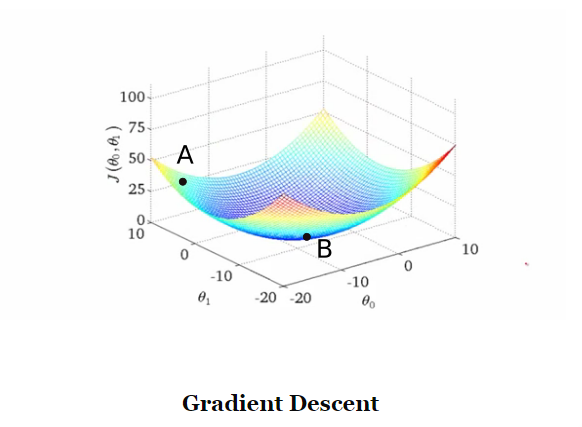
\includegraphics[width =.9 \textwidth,height=.48\textheight]{GD.png}
\end{frame}

\begin{frame}
\frametitle{Gradient Descent}
Assume $\mathbf{f}(\mathbf{x})$ is a continuously differentiable function.Given $\epsilon$ with a small enough absolute value,according to the Taylor's expansion formula,we get the following approximation:\\
\centerline{$\mathbf{f}(\mathbf{x}+\epsilon)\approx\mathbf{f}(\mathbf{x})+\epsilon\mathbf{f}'(\mathbf{x})$}
The gradient of a one-dimensional function is a scalar, also known as a derivative.Next, find a constant
$\eta>0$,to make $|\eta\mathbf{f}'(\mathbf{x})|$ sufficiently small so that we can replace $\epsilon$ with 
$-\eta\mathbf{f}(\mathbf{x})$ and get:\\
\centerline{$\mathbf{f}\Big(\mathbf{x}-\eta\mathbf{f}'\big(\mathbf{x}\big)\Big)\approx\mathbf{f}(\mathbf{x})\
-\eta\mathbf{f}'(\mathbf{x})^2$}
If the derivative $\mathbf{f}'(\mathbf{x})\neq0$,then $\eta\mathbf{f}'(\mathbf{x})^2>0$,so\\
\centerline{$\mathbf\
{f}\Big(\mathbf{x}-\eta\mathbf{f}'\big(\mathbf{x}\big)\Big)\leq\mathbf{f}(\mathbf{x})$}
This means,if we use\\
\centerline{$\mathbf{x}\leftarrow\mathbf{x}-\eta\mathbf{f}'(\mathbf{x})$}
to iterate $\mathbf{x}$,the value of function $\mathbf{f}(\mathbf{x})$ might decline.
\end{frame}

\begin{frame}
\frametitle{Gradient Descent}
The positive $\eta$ in the the above gradient descent algorithm is usually called the learning rate.
This is a hyper-parameter and needs to be set manually. If we use a learning rate that is too small
it will cause $\mathbf{x}$ to update at a very slow speed, requiring more iterations to get a better solution.
Now assume $f(x)=x^2,\eta=0.05,iterations=10$\\
\begin{figure}
	\begin{minipage}[t]{0.49\linewidth} % 如果一行放2个图,用0.5,如果3个图,用0.33
		\centering
		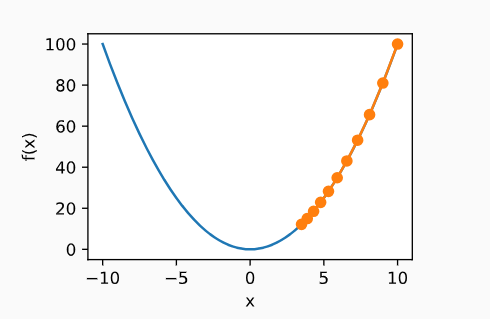
\includegraphics[width= \textwidth]{n05.png}
		\caption{$\eta$=0.05}
		\label{fig:side:a}
	\end{minipage}%
	\begin{minipage}[t]{0.49\linewidth}
		\centering
		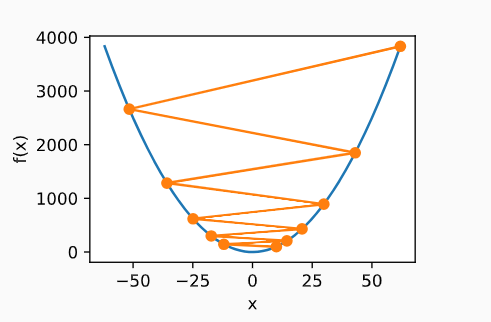
\includegraphics[width= \textwidth]{n11.png}
		\caption{$\eta$=1.1}
		%\label{fig:side:b}
	\end{minipage}
\end{figure}
\end{frame}

\section{Batch Gradient Descent(BGD)}
\subsection{Batch Gradient Descent(BGD)}

\begin{frame}
\frametitle{Batch Gradient Descent}
	\begin{block}{Basic idea:}
	Parameters are updated after computing the gradient of error with respect to the entire training set.
	\end{block}
\end{frame}

\subsection{Example}
\begin{frame}
\frametitle{Example}
test-BGD.py,try to set the different learning rate to see the output:\\
~\\
\url{https://github.com/IEC-lab/MachineLearning2019/blob/master/GD/test-BGD.py}
\end{frame}

\subsection{Summary}
\begin{frame}
\frametitle{Summary for BGD}
Upsides:
	\begin{itemize}
	\item Fewer updates to the model means this variant of gradient descent is more computationally efficient than stochastic gradient descent.
	\item The decreased update frequency results in a more stable error gradient and may result in a more stable convergence on some problems.
	\item The separation of the calculation of prediction errors and the model update lends the algorithm to parallel processing based implementations.
	\end{itemize}
\end{frame}

\begin{frame}
\frametitle{Summary for BGD}
Downsides:
	\begin{itemize}
	\item The more stable error gradient may result in premature convergence of the model to a less optimal set of parameters.
	\item The updates at the end of the training epoch require the additional complexity of accumulating prediction errors across all training examples.
	\item Commonly, batch gradient descent is implemented in such a way that it requires the entire training dataset in memory and available to the algorithm.
	\item Model updates, and in turn training speed, may become very slow for large datasets.
	\end{itemize}
\end{frame}

\section{Stochastic Gradient Descent(SGD)}
\subsection{Stochastic Gradient Descent(SGD)}

\begin{frame}
\frametitle{Stochastic Gradient Descent}
	\begin{block}{Quiz}
	In Machine Learning,the training set is enormous and no simple formulas exist, evaluating the sums of 		gradients becomes very expensive, because evaluating the gradient requires evaluating all the summand functions' 	gradients.
	How to minimize the computational cost at every iteration? 
	\end{block}
\end{frame}

\begin{frame}
\frametitle{Stochastic Gradient Descent}
\begin{block}{Solution}
Samples a subset of the training set at every step instead of the whole set.Parameters are updated after computing the gradient of error with respect to a single training example.
\end{block}
In pseudocode, stochastic gradient descent can be presented as follows:\\
\begin{itemize}
\item Choose an initial vector of parameters $x$ and learning rate $\eta$
\item Repeat until an approximate minimum is obtained:
\begin{itemize}
\item Randomly shuffle examples in the training set.
\item For $i$=1,2,...,n,do:
\begin{itemize}
\item $x=x-\eta f'_i(x)$
\end{itemize}
\end{itemize}
\end{itemize}
\end{frame}

\subsection{Example}

\begin{frame}
\frametitle{Example}
We can add random noise with a mean of 0 to the gradient to simulate a SGD:
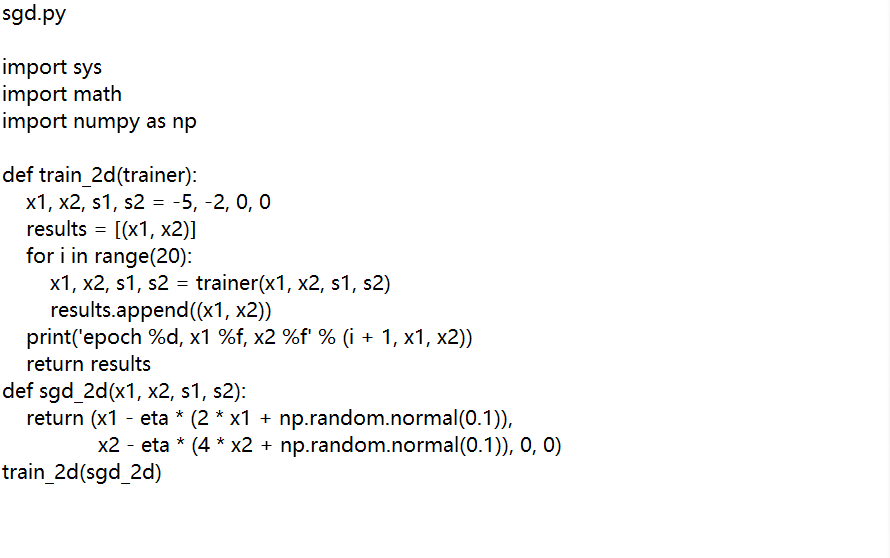
\includegraphics[width= \textwidth]{sgd1.png}
\end{frame}

\begin{frame}
\frametitle{Example}
\begin{figure}
\begin{minipage}[t]{\linewidth}
\centering
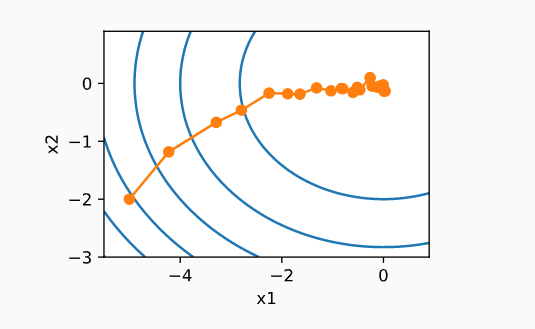
\includegraphics[width= .6\textwidth]{SGD.png}
\caption{epoch=20}
\end{minipage}
\end{figure}
As we can see,the iterative trajectory of the independent variable in the SGD is more tortuous than in the gradient descent.This is due to the noise added in the experiment, which reduced the accuracy of the simulated stochastic gradient. In practice, such noise usually comes from individual examples in the training data set.
\end{frame}

\begin{frame}
\frametitle{Example}
test-SGD.py:\\
~\\
\url{https://github.com/IEC-lab/MachineLearning2019/blob/master/GD/test-SGD.py}
\end{frame}

\subsection{Summary}
\begin{frame}
\frametitle{Summary for SGD}
Upsides:
\begin{itemize}
	\item The frequent updates immediately give an insight into the performance of the model and the rate of improvement.
	\item This variant of gradient descent may be the simplest to understand and implement, especially for beginners.
	\item The increased model update frequency can result in faster learning on some problems.
	\item The noisy update process can allow the model to avoid local minima (e.g. premature convergence).
\end{itemize}
\end{frame}

\begin{frame}
\frametitle{Summary for SGD}
Downsides:
\begin{itemize}
	\item Updating the model so frequently is more computationally expensive than other configurations of gradient descent, taking significantly longer to train models on large datasets.
	\item The frequent updates can result in a noisy gradient signal, which may cause the model parameters and in turn the model error to jump around (have a higher variance over training epochs).
	\item The noisy learning process down the error gradient can also make it hard for the algorithm to settle on an error minimum for the model.
\end{itemize}
\end{frame}

\section{Mini-batch Stochastic Gradient Descent}

\subsection{Mini-batch Stochastic Gradient Descent}

\begin{frame}
\frametitle{Mini-batch Stochastic Gradient Descent}
	\begin{block}{Basic idea:}
	Mini-batch gradient descent seeks to find a balance between the robustness of stochastic gradient descent and the efficiency of batch gradient descent. Parameters are updated after computing the gradient of error with respect to a subset of the training set
	\end{block}
\end{frame}

\begin{frame}
\frametitle{Mini-batch Stochastic Gradient Descent}
In pseudocode, Mini stochastic gradient descent can be presented as follows:\\
Let theta = model parameters and max\_iters = number of epochs.\\
for itr = 1, 2, 3,..., max\_iters:\\
\quad for mini\_batch(X\_mini, y\_mini):
	\begin{itemize}
	\item Forward Pass on the batch X\_mini:
		\begin{itemize}
		\item Make predictions on the mini-batch
		\item Compute error in predictions $(J(theta))$ with the current values of the parameters
		\end{itemize}
	\end{itemize}
	\begin{itemize}
	\item Backward Pass:
		\begin{itemize}
		\item Compute gradient$(theta)$ = partial derivative of $J(theta)$ w.r.t. $theta$
		\end{itemize}
	\end{itemize}
	\begin{itemize}
	\item Update parameters:
		\begin{itemize}
		\item $theta = theta – learning\_rate*gradient(theta)$
		\end{itemize}
	\end{itemize}
\end{frame}

\subsection{Comparison with BGD\&SGD}
\begin{frame}
\frametitle{Comparison with BGD\&SGD}
\begin{figure}
	\begin{minipage}[t]{0.6\linewidth} % 如果一行放2个图,用0.5,如果3个图,用0.33
		\centering
		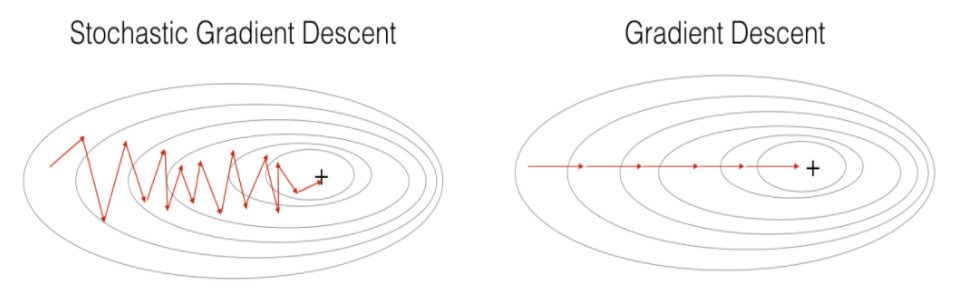
\includegraphics[width= \textwidth]{c1.png}
		\caption{SGD vs BGD}
		\label{fig:side:a}
	\end{minipage}%

	\begin{minipage}[t]{0.6\linewidth}
		\centering
		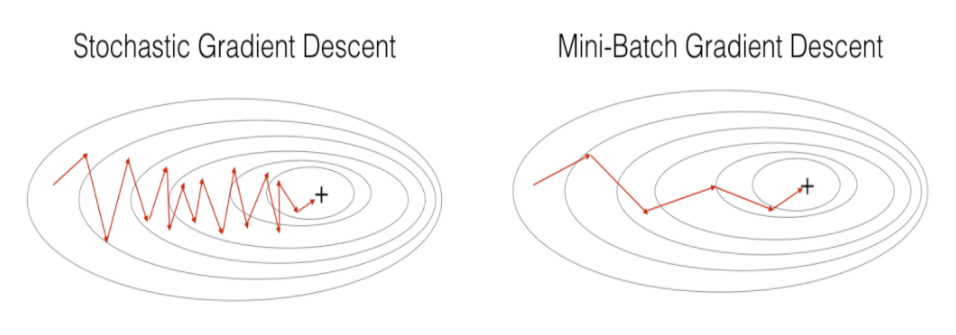
\includegraphics[width= \textwidth]{c2.png}
		\caption{SGD vs MSGD}
		%\label{fig:side:b}
	\end{minipage}
\end{figure}
\end{frame}

\begin{frame}
\frametitle{Comparison with BGD\&SGD}
\begin{block}{}
In summary, the difference between gradient descent, mini-batch gradient descent, and stochastic gradient descent is the number of examples you use to perform one update step. With a well tuned mini-batch size, it outperforms gradient descent or stochastic gradient descent.
\end{block}
\end{frame}

\subsection{How to Configure Mini-Batch Gradient Descent}
\begin{frame}
\frametitle{Batch size}
Mini-batch sizes, commonly called "batch sizes" for brevity, are often tuned to an aspect of the computational architecture on which the implementation is being executed. Such as a power of two that fits the memory requirements of the GPU or CPU hardware like 32, 64, 128, 256, and so on.\\
~\\
Batch size is a slider on the learning process.
\begin{itemize}
\item Small values give a learning process that converges quickly at the cost of noise in the training process.
\item Large values give a learning process that converges slowly with accurate estimates of the error gradient.
\end{itemize}
\end{frame}

\begin{frame}
\frametitle{Configure batch size}
\begin{block}{}
Tip1:
\begin{itemize}
\item A good default for batch size might be 32. \quad-Revisiting Small Batch Training for Deep Neural Networks, 2018.
\end{itemize}
~\\
Tip2:
\begin{itemize}
\item  It is a good idea to review learning curves of model validation error against training time with different batch sizes when tuning the batch size. 
\end{itemize}
Tip3:
\begin{itemize}
\item  Tune batch size and learning rate after tuning all other hyperparameters. 
\end{itemize}
\end{block}
\end{frame}

\subsection{Example}
\begin{frame}
\frametitle{Example}
test-MSGD.py:\\
~\\
\url{https://github.com/IEC-lab/MachineLearning2019/blob/master/GD/test-MSGD.py}
\end{frame}

\subsection{Summary}
\begin{frame}
\frametitle{Summary for MSGD}
Upsides:
\begin{itemize}
	\item The model update frequency is higher than batch gradient descent which allows for a more robust convergence, avoiding local minima.
	\item The batched updates provide a computationally more efficient process than stochastic gradient descent.
	\item The batching allows both the efficiency of not having all training data in memory and algorithm implementations.
\end{itemize}
\end{frame}

\begin{frame}
\frametitle{Summary for MSGD}
Downsides:
\begin{itemize}
	\item Mini-batch requires the configuration of an additional “mini-batch size” hyperparameter for the learning algorithm.
	\item Error information must be accumulated across mini-batches of training examples like batch gradient descent.
\end{itemize}
\end{frame}

\begin{frame}
\begin{center}
\huge The end!
\end{center}
\end{frame}
%
%\end{CJK*}

\end{document}
